\newpage

\chapter{Lezione 3: 14/03/2025}

Abbiamo visto che un tensore controvariante è un tensore che passa da un sistema di riferimento normale ad uno "prime", con una trasformazione del tipo:

$$
V'^j = V^i \cdot \dfrac{\partial x'^j}{\partial x^i}
$$

Mentre un tensore covariante è un tensore che passa da un sistema di riferimento "prime" ad uno normale, con una trasformazione del tipo:

$$
V'_j = V_i \cdot \dfrac{\partial x^i}{\partial x'^j}
$$

Abbiamo visto anche il concetto di curvatura partendo dalla derivata del versore tangente ad una curva, partendo da questo, definiamo la curvatura rispetto ad una superficie.

\section{Curvatura di una Superficie}

\begin{minipage}[H]{0.55\textwidth}
    L'estensione della curvatura a una superficie si basa sulla scelta di un punto $P$ e del versore normale $\hat{n}$ in $P$. Il vettore tangente $\bar v$ in $P$ e quello normale $\hat{n}$ individuano un piano che interseca la superficie, generando una curva la cui \textbf{curvatura} in $P$ è espressa da:

    $$k = \pm \tfrac{1}{R}$$

    Il segno dipende dal lato su cui giace il centro di curvatura $C$ rispetto a $\hat{n}$. La convenzione sul segno non altera la sostanza del concetto di curvatura.
\end{minipage}%
\hspace{0.04\textwidth}
\begin{minipage}{0.4\textwidth}
    \begin{figure}[H]
        \centering
        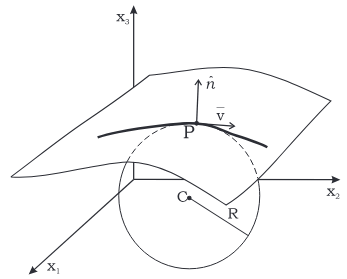
\includegraphics[width=\textwidth]{assets/surface_curv.png}
        \caption{Curvatura di una Superficie}
        \label{fig:curvatura_superficie}
    \end{figure}
\end{minipage}

In un cilindro si individuano due direzioni ortogonali, dove si ottengono i valori estremo di $k$ (chiamati $k_1$ e $k_2$), detti curvature principali. In generale, ciò vale per qualunque superficie regolare. Definiamo la curvatura di Gauss $K$ come il prodotto $k_1 \cdot k_2$, evidenziando che $K$ non dipende dalla convenzione scelta per il segno di $k$.

\begin{figure}[H]
    \centering
    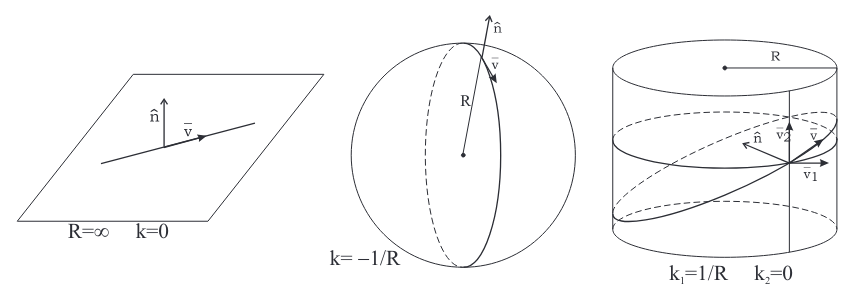
\includegraphics[width=0.5\textwidth]{assets/ex_curvature.png}
    \caption{Curvatura di un piano, di una sfera e di un cilindro}
    \label{fig:ex_curvature}
\end{figure}

Una curva è \textbf{geodetica} quando la sua lunghezza è stazionaria per piccole variazioni agli estremi. 

Immaginate di avere un elastico teso tra due punti: se lo perturbate, le perfurbazioni si annullano agli estremi.

$$
\bar r (s) = \vec r(U^i) = \vec r(U^i(t))
$$

\begin{observationblock}[Geodetica]
    Anche i tragitti più lunghi che collegano due punti formano delle geodetiche, non solo i tragitti più brevi.
\end{observationblock}

Se ricordiamo che $ds^2 = g_{jk} du^j du^k$, espresse le $u^i$ in forma parametrica tramite il parametro $t$ (che non sará
necessariamente il tempo) avremo:

$$
g_{jk}\dfrac{du^j}{dt} \dfrac{du^k}{dt} dt^2 
=
(g_{jk} \dot u^j \dot u^k) dt^2
$$

Detta $L(u^i, \dot u^i, t) = \sqrt{g_{jk} \dot u^j \dot u^k} = \sqrt{F}$, (con le $g_{jk} = g_{jk}(u^i)$ e $\dot u^i = \tfrac{du^i}{dt}$) la lunghezza di una curva tra $P_1$ e $P_2$ sarà:

$$
S = \int_{P_1}^{P_2} L dt = \int_{P_1}^{P_2} ds
$$

Per trovare la condizione che $S$ sia stazionario si usano le \textbf{equazioni di Eulero-Lagrange}:

$$
\dfrac{dL}{du'} = \dfrac{d}{dt} \left( \dfrac{\partial L}{\partial \dot u^i} \right) 
\quad \Rightarrow \quad
\dfrac{dL}{du'} - \dfrac{d}{dt} \left( \dfrac{\partial L}{\partial \dot u^i} \right) = 0
$$

Risolviamo l'equazione di Eulero Lagrange per $u^i$:

$$
\dfrac{\partial g_{jk}\dot u^j u^k}{\partial u^i} =
\dfrac{\partial g_{js}}{\partial u^i}u^j \dot u^k + \dfrac{\partial \dot u^j}{\partial u^i}g_{jk}u^k + \dfrac{\partial u^k}{\partial u^i}g_{jk}\dot u^j
$$

$$
\dfrac{\partial \sqrt F}{\partial u^i}
- 
\dfrac d{dt} \left( \dfrac{\partial \sqrt F}{\partial \dot u^i} \right) 
= 
\dfrac 1 {2\sqrt F} \dfrac{\partial g_{jk}}{\partial u^i} \dot u^j \dot u^k 
- 
\dfrac d{dt} \left[ \dfrac 1 {2\sqrt F} \dfrac{\partial (g_{jk} \dot u^j \dot u^k)}{\partial \dot u^i} \right]
= 0
$$

Poichè 
$
\tfrac {\partial g_{jk} \dot u^j \dot u^k}{\partial \dot u^i} = g_{ik} \dot u^k + g_{ij} \dot u^j
$
riscriviamo:

$$
\dfrac{1}{2\sqrt F} \dfrac{\partial g_{jk}}{\partial \dot u^i} \dot u^j \dot u^k - \dfrac{d}{dt} \left[ \dfrac{1}{2\sqrt F} \underbrace{(g_{ik} \dot u^k + g_{ij} \dot u^j)}_{=\ 2g_{ji}\dot u^j} \right] = 0
$$

ma $g_{ik}\dot{u}^k + g_{ij}\dot{u}^j = 2\,g_{ij}\dot{u}^j$ per la simmetria di $g_{ij}$ e per il fatto che $k$ e $j$ sono indici muti (sommati) e si possono scambiare; avremo quindi:

$$
\dfrac 1{2\sqrt F} \dfrac{\partial g_{jk}}{\partial \dot u^i} \dot u^j \dot u^k - \dfrac d{dt} \left[ \dfrac 1 {\sqrt F} g_{ji} \dot u^j \right] = 0
$$

$$
\dfrac 1{2\sqrt F} \dfrac{\partial g_{jk}}{\partial \dot u^i} \dot u^j \dot u^k
-
\left\{
\underbrace{
- \dfrac 1{2 F^{3/2}} \dfrac {dF}{dt} g_{ji} \dot u^j 
}_{= \ 0}
+ \dfrac 1{\sqrt F}
\left(
    \dfrac{\partial g_{ji}}{\partial u^l } \dot u^l \dot u^j + g_{ji} \ddot u^j
\right)
\right\}
= 0
$$

$$
\dfrac 12 
\left[
    \dfrac{\partial g_{ji}}{\partial \dot u^l} + \dfrac{\partial g_{li}}{\partial \dot u^j}
\right]
\dot u^j \dot u^l
=
\dfrac {\partial g_{ji}}{\partial u^l} \dot u^l \dot u^j
=
\dfrac {\partial g_{li}}{\partial u^j} \dot u^j \dot u^l
$$

$$
g_{ji} \ddot u^j + \dfrac 12
\left[
    \dfrac{\partial g_{ji}}{\partial u^k} \dot u^k \dot u^j
    +
    \dfrac{\partial g_{ki}}{\partial u^j} \dot u^k \dot u^j
    -
    \dfrac{\partial g_{jk}}{\partial u^i} \dot u^j \dot u^k
\right]
=
g_{ji} \ddot u^j +
\left[
    \partial{g_{ji}}{\partial u^l} \dot u^l \dot u^j - \dfrac 12 \dfrac{\partial g_{jk}}{\partial u^i} \dot u^j \dot u^k
\right] 
= 0
$$

\dots

$$
\dfrac 12 g^{il} \left[ \dfrac{\partial g_{lj}}{\partial u^k} + \dfrac{\partial g_{lk}}{\partial u^j} - \dfrac{\partial g_{jk}}{\partial u^l} \right]
$$

Dove $\Gamma^l_{jk}$ è detto \textbf{\textit{connessione affine}}, o \textbf{\textit{simbolo di Christoffel di 2° tipo}}.

\dots

Arriviamo finalmente all'\textbf{equazione delle geodetiche}:

$$
\boxed{
\dfrac{d^2u^l}{ds^2} + \Gamma^l_{jk} \dfrac{du^j}{ds} \dfrac{du^k}{ds} = 0
}
$$